\documentclass[a4paper,12pt,openright]{book}
%\documentclass[a4paper, 12pt, openright, draft]{book}  Nalogo preverite tudi z opcijo draft, ki pokaže, katere vrstice so predolge! Pozor, v draft opciji, se slike ne pokažejo!
 
\usepackage[utf8]{inputenc}
\usepackage[slovene,english]{babel}
\usepackage[pdftex]{graphicx}
\usepackage{fancyhdr}
\usepackage{amssymb}
\usepackage{amsmath}           % eqref, npr.
\usepackage{hyperxmp}
\usepackage[hyphens]{url}
\usepackage{csquotes}
\usepackage[pdftex, colorlinks=true,
citecolor=black, filecolor=black, 
linkcolor=black, urlcolor=black,
pdfproducer={LaTeX}, pdfcreator={LaTeX}]{hyperref}

\usepackage{color}
\usepackage{soul}
\usepackage{array}
\usepackage{tikz}
\usepackage{listings}

\tikzstyle{arrow} = [thick,->,>=stealth]

\definecolor{codegreen}{rgb}{0,0.6,0}
\definecolor{codegray}{rgb}{0.5,0.5,0.5}
\definecolor{codepurple}{rgb}{0.58,0,0.82}
\definecolor{backcolour}{rgb}{0.95,0.95,0.92}

\lstset{
	backgroundcolor=\color{backcolour},   
    commentstyle=\color{codegreen},
    keywordstyle=\color{magenta},
    numberstyle=\tiny\color{codegray},
    stringstyle=\color{codepurple},
    basicstyle=\ttfamily\footnotesize,
	breaklines=true,
	tabsize=4,
	numbers=left
}

\usepackage[
backend=biber,
style=numeric,
sorting=nty,
]{biblatex}

\addbibresource{bibliography.bib}


%%%%%%%%%%%%%%%%%%%%%%%%%%%%%%%%%%%%%%%%
%	DIPLOMA INFO
%%%%%%%%%%%%%%%%%%%%%%%%%%%%%%%%%%%%%%%%
\newcommand{\ttitle}{Primerjava sistemskih klicev Linux in Windows}
\newcommand{\ttitleEn}{The comparison of Linux and Windows system calls}
\newcommand{\tsubject}{\ttitle}
\newcommand{\tsubjectEn}{\ttitleEn}
\newcommand{\tauthor}{Miha Meglič}
\newcommand{\tkeywords}{sistemski klic, linux, windows, operacijski sistem}
\newcommand{\tkeywordsEn}{system call, linux, windows, operating system}

%%%%%%%%%%%%%%%%%%%%%%%%%%%%%%%%%%%%%%%%
%	HYPERREF SETUP
%%%%%%%%%%%%%%%%%%%%%%%%%%%%%%%%%%%%%%%%
\hypersetup{pdftitle={\ttitle}}
\hypersetup{pdfsubject=\ttitleEn}
\hypersetup{pdfauthor={\tauthor}}
\hypersetup{pdfkeywords=\tkeywordsEn}

%%%%%%%%%%%%%%%%%%%%%%%%%%%%%%%%%%%%%%%%
% postavitev strani
%%%%%%%%%%%%%%%%%%%%%%%%%%%%%%%%%%%%%%%%  

\addtolength{\marginparwidth}{-20pt} % robovi za tisk
\addtolength{\oddsidemargin}{40pt}
\addtolength{\evensidemargin}{-40pt}

\renewcommand{\baselinestretch}{1.3} % ustrezen razmik med vrsticami
\setlength{\headheight}{15pt}        % potreben prostor na vrhu
\renewcommand{\chaptermark}[1]%
{\markboth{\MakeUppercase{\thechapter.\ #1}}{}} \renewcommand{\sectionmark}[1]%
{\markright{\MakeUppercase{\thesection.\ #1}}} \renewcommand{\headrulewidth}{0.5pt} \renewcommand{\footrulewidth}{0pt}
\fancyhf{}
\fancyhead[LE,RO]{\sl \thepage} 
%\fancyhead[LO]{\sl \rightmark} \fancyhead[RE]{\sl \leftmark}
\fancyhead[RE]{\sc \tauthor}
\fancyhead[LO]{\sc Diplomska naloga}


\newcommand{\BibLaTeX}{{\sc Bib}\LaTeX}
\newcommand{\BibTeX}{{\sc Bib}\TeX}

%%%%%%%%%%%%%%%%%%%%%%%%%%%%%%%%%%%%%%%%
% naslovi
%%%%%%%%%%%%%%%%%%%%%%%%%%%%%%%%%%%%%%%%  

\newcommand{\autfont}{\Large}
\newcommand{\titfont}{\LARGE\bf}
\newcommand{\clearemptydoublepage}{\newpage{\pagestyle{empty}\cleardoublepage}}
\setcounter{tocdepth}{1}

%%%%%%%%%%%%%%%%%%%%%%%%%%%%%%%%%%%%%%%%
% konstrukti
%%%%%%%%%%%%%%%%%%%%%%%%%%%%%%%%%%%%%%%%  
\newtheorem{izrek}{Izrek}[chapter]
\newtheorem{trditev}{Trditev}[izrek]
\newenvironment{dokaz}{\emph{Dokaz.}\ }{\hspace{\fill}{$\Box$}}


%%%%%%%%%%%%%%%%%%%%%%%%%%%%%%%%%%%%%%%%%%%%%%%%%%%%%%%%%%%%%%%%%%%%%%%%%%%%%%%
%% PDF-A
%%%%%%%%%%%%%%%%%%%%%%%%%%%%%%%%%%%%%%%%%%%%%%%%%%%%%%%%%%%%%%%%%%%%%%%%%%%%%%%

%%%%%%%%%%%%%%%%%%%%%%%%%%%%%%%%%%%%%%%% 
% define medatata
%%%%%%%%%%%%%%%%%%%%%%%%%%%%%%%%%%%%%%%% 
\def\Title{\ttitle}
\def\Author{\tauthor, miha@meglic.dev}
\def\Subject{\ttitleEn}
\def\Keywords{\tkeywordsEn}

%%%%%%%%%%%%%%%%%%%%%%%%%%%%%%%%%%%%%%%% 
% \convertDate converts D:20080419103507+02'00' to 2008-04-19T10:35:07+02:00
%%%%%%%%%%%%%%%%%%%%%%%%%%%%%%%%%%%%%%%% 
\def\convertDate{%
    \getYear
}

{\catcode`\D=12
 \gdef\getYear D:#1#2#3#4{\edef\xYear{#1#2#3#4}\getMonth}
}
\def\getMonth#1#2{\edef\xMonth{#1#2}\getDay}
\def\getDay#1#2{\edef\xDay{#1#2}\getHour}
\def\getHour#1#2{\edef\xHour{#1#2}\getMin}
\def\getMin#1#2{\edef\xMin{#1#2}\getSec}
\def\getSec#1#2{\edef\xSec{#1#2}\getTZh}
\def\getTZh +#1#2{\edef\xTZh{#1#2}\getTZm}
\def\getTZm '#1#2'{%
    \edef\xTZm{#1#2}%
    \edef\convDate{\xYear-\xMonth-\xDay T\xHour:\xMin:\xSec+\xTZh:\xTZm}%
}

%\expandafter\convertDate\pdfcreationdate 

%%%%%%%%%%%%%%%%%%%%%%%%%%%%%%%%%%%%%%%%
% get pdftex version string
%%%%%%%%%%%%%%%%%%%%%%%%%%%%%%%%%%%%%%%% 
\newcount\countA
\countA=\pdftexversion
\advance \countA by -100
\def\pdftexVersionStr{pdfTeX-1.\the\countA.\pdftexrevision}


%%%%%%%%%%%%%%%%%%%%%%%%%%%%%%%%%%%%%%%%
% XMP data
%%%%%%%%%%%%%%%%%%%%%%%%%%%%%%%%%%%%%%%%  
\usepackage{xmpincl}
%\includexmp{pdfa-1b}

%%%%%%%%%%%%%%%%%%%%%%%%%%%%%%%%%%%%%%%%
% pdfInfo
%%%%%%%%%%%%%%%%%%%%%%%%%%%%%%%%%%%%%%%%  
\pdfinfo{%
    /Title    (\ttitle)
    /Author   (\tauthor, miha@meglic.dev)
    /Subject  (\ttitleEn)
    /Keywords (\tkeywordsEn)
    /ModDate  (\pdfcreationdate)
    /Trapped  /False
}

%%%%%%%%%%%%%%%%%%%%%%%%%%%%%%%%%%%%%%%%
% znaki za copyright stran
%%%%%%%%%%%%%%%%%%%%%%%%%%%%%%%%%%%%%%%%  

\newcommand{\CcImageCc}[1]{%
	
\includegraphics[scale=#1]{resources/cc_cc_30.pdf}%
}
\newcommand{\CcImageBy}[1]{%
	
\includegraphics[scale=#1]{resources/cc_by_30.pdf}%
}
\newcommand{\CcImageSa}[1]{%
	
\includegraphics[scale=#1]{resources/cc_sa_30.pdf}%
}

%%%%%%%%%%%%%%%%%%%%%%%%%%%%%%%%%%%%%%%%%%%%%%%%%%%%%%%%%%%%%%%%%%%%%%%%%%%%%%%
%%%%%%%%%%%%%%%%%%%%%%%%%%%%%%%%%%%%%%%%%%%%%%%%%%%%%%%%%%%%%%%%%%%%%%%%%%%%%%%

\begin{document}
\selectlanguage{slovene}
\frontmatter
\setcounter{page}{1} %
\renewcommand{\thepage}{}       % preprečimo težave s številkami strani v kazalu

%%%%%%%%%%%%%%%%%%%%%%%%%%%%%%%%%%%%%%%%
%naslovnica
\thispagestyle{empty}%
\begin{center}
	{\large\sc Univerza v Ljubljani\\
		Fakulteta za računalništvo in informatiko\\
	}
	\vskip 10em
	{\autfont \tauthor\par}
	{\titfont \ttitle \par}
	{\vskip 3em \textsc{DIPLOMSKO DELO\\[5mm]
		UNIVERZITETNI  ŠTUDIJSKI PROGRAM\\ PRVE STOPNJE\\ RAČUNALNIŠTVO IN INFORMATIKA}\par}
	\vfill\null
	{\large \textsc{Mentor}: doc. dr. Jurij Mihelič\par}
	{\vskip 2em \large Ljubljana, \the\year \par}
\end{center}
% prazna stran
%\clearemptydoublepage      
% izjava o licencah itd. se izpiše na hrbtni strani naslovnice

%%%%%%%%%%%%%%%%%%%%%%%%%%%%%%%%%%%%%%%%
%copyright stran
%%%%%%%%%%%%%%%%%%%%%%%%%%%%%%%%%%%%%%%%
\newpage
\thispagestyle{empty}

\vspace*{5cm}
{\small \noindent
	To delo je ponujeno pod licenco \textit{Creative Commons Priznanje avtorstva-Deljenje pod enakimi pogoji 2.5 Slovenija} (ali novej\v so razli\v cico).
	To pomeni, da se tako besedilo, slike, grafi in druge sestavine dela kot tudi rezultati diplomskega dela lahko prosto distribuirajo,
	reproducirajo, uporabljajo, priobčujejo javnosti in predelujejo, pod pogojem, da se jasno in vidno navede avtorja in naslov tega
	dela in da se v primeru spremembe, preoblikovanja ali uporabe tega dela v svojem delu, lahko distribuira predelava le pod
	licenco, ki je enaka tej.
	Podrobnosti licence so dostopne na spletni strani \href{http://creativecommons.si}{creativecommons.si} ali na Inštitutu za
	intelektualno lastnino, Streliška 1, 1000 Ljubljana.
																																																																							
	\vspace*{1cm}
	\begin{center}% 0.66 / 0.89 = 0.741573033707865
		\CcImageCc{0.741573033707865}\hspace*{1ex}\CcImageBy{1}\hspace*{1ex}\CcImageSa{1}%
	\end{center}
}

\vspace*{1cm}
{\small \noindent
	Izvorna koda diplomskega dela, njeni rezultati in v ta namen razvita programska oprema je ponujena pod licenco GNU General Public License,
	različica 3 (ali novejša). To pomeni, da se lahko prosto distribuira in/ali predeluje pod njenimi pogoji.
	Podrobnosti licence so dostopne na spletni strani \url{http://www.gnu.org/licenses/}.
}

\vfill
\begin{center} 
	\ \\ \vfill
	{\em
		Besedilo je oblikovano z urejevalnikom besedil \LaTeX.}
\end{center}

% prazna stran
\clearemptydoublepage

%%%%%%%%%%%%%%%%%%%%%%%%%%%%%%%%%%%%%%%%
% stran 3 med uvodnimi listi
\thispagestyle{empty}
\
\vfill

\bigskip
\noindent\textbf{Kandidat:} \tauthor\\
\noindent\textbf{Naslov:} \ttitle\\
\noindent\textbf{Vrsta naloge:} Diplomska naloga na univerzitetnem programu prve stopnje Računalništvo in informatika \\
\noindent\textbf{Mentor:} doc. dr. Jurij Mihelič

\bigskip
\noindent\textbf{Opis:}\\
Besedilo teme diplomskega dela študent prepiše iz študijskega informacijskega sistema, kamor ga je vnesel mentor. 
V nekaj stavkih bo opisal, kaj pričakuje od kandidatovega diplomskega dela. 
Kaj so cilji, kakšne metode naj uporabi, morda bo zapisal tudi ključno literaturo.

\bigskip
\noindent\textbf{Title:} \ttitleEn

\bigskip
\noindent\textbf{Description:}\\
opis diplome v angleščini

\vfill



\vspace{2cm}

% prazna stran
\clearemptydoublepage

% zahvala
\thispagestyle{empty}\mbox{}\vfill\null\it%
\noindent
Na tem mestu zapišite, komu se zahvaljujete za pomoč pri izdelavi diplomske naloge oziroma pri vašem študiju nasploh. Pazite, da ne boste koga pozabili. Utegnil vam bo zameriti. Temu se da izogniti tako, da celotno zahvalo izpustite.
\rm\normalfont

% prazna stran
\clearemptydoublepage


%%%%%%%%%%%%%%%%%%%%%%%%%%%%%%%%%%%%%%%%
% kazalo
\pagestyle{empty}
\def\thepage{}% preprečimo težave s številkami strani v kazalu
\tableofcontents{}


% prazna stran
\clearemptydoublepage

%%%%%%%%%%%%%%%%%%%%%%%%%%%%%%%%%%%%%%%%
% seznam kratic

\chapter*{Seznam uporabljenih kratic}

\noindent\begin{tabular}{p{0.11\textwidth}|p{.39\textwidth}|p{.39\textwidth}}    % po potrebi razširi prvo kolono tabele na račun drugih dveh!
{\bf kratica} & {\bf angleško}                     & {\bf slovensko}                         \\
\hline
{\bf OS}      & Operating System                    & operacijski sistem                      \\
{\bf API}     & Application Programming Interface   & vmesnik uporabniškega programa         \\
{\bf POSIX}   & Portable Operating System Interface & Prenosni Vmesnik za Operacijske Sisteme \\
{\bf SUS}     & Single UNIX Specification           & Enotna UNIX specifikacija               \\
\end{tabular}


% prazna stran
\clearemptydoublepage

%%%%%%%%%%%%%%%%%%%%%%%%%%%%%%%%%%%%%%%%
% povzetek
\addcontentsline{toc}{chapter}{Povzetek}
\chapter*{Povzetek}

\noindent\textbf{Naslov:} \ttitle
\bigskip

\noindent\textbf{Avtor:} \tauthor
\bigskip

%\noindent\textbf{Povzetek:} 
\noindent V vzorcu je predstavljen postopek priprave diplomskega dela z uporabo okolja \LaTeX. Vaš povzetek mora sicer vsebovati približno 100 besed, ta tukaj je odločno prekratek.
Dober povzetek vključuje: (1) kratek opis obravnavanega problema, (2) kratek opis vašega pristopa za reševanje tega problema in (3) (najbolj uspešen) rezultat ali prispevek diplomske naloge.

\bigskip

\noindent\textbf{Ključne besede:} \tkeywords.
% prazna stran
\clearemptydoublepage

%%%%%%%%%%%%%%%%%%%%%%%%%%%%%%%%%%%%%%%%
% abstract
\selectlanguage{english}
\addcontentsline{toc}{chapter}{Abstract}
\chapter*{Abstract}

\noindent\textbf{Title:} \ttitleEn
\bigskip

\noindent\textbf{Author:} \tauthor
\bigskip

%\noindent\textbf{Abstract:} 
\noindent This sample document presents an approach to typesetting your BSc thesis using \LaTeX. 
A proper abstract should contain around 100 words which makes this one way too short.
\bigskip

\noindent\textbf{Keywords:} \tkeywordsEn.
\selectlanguage{slovene}
% prazna stran
\clearemptydoublepage

%%%%%%%%%%%%%%%%%%%%%%%%%%%%%%%%%%%%%%%%
\mainmatter
\setcounter{page}{1}
\pagestyle{fancy}

\chapter{Uvod}


\chapter{Pregled področja}

Moderni računalniki vsebujejo mnogo različnih komponent -- centralno procesno enoto, pomnilnik in vhodno-izhodne naprave.
Pri takem obsegu in kompleksnosti računalniških sistemov je praktično nepredstavljivo, da bi vsak programer poznal vse podrobnosti delovanja vseh komponent.
Zato se je pojavila potreba po programu, katerega naloga je upravljanje z viri sistema in abstrakcija dostopa do le teh -- \textbf{operacijski sistem}.

\section{Operacijski sistem}

Operacijski sistem iz uporabnikove perspektive stoji med aplikacijami in strojno opremo, kot vidimo na sliki \ref{fig:computer_system_components}.

\begin{figure}[h!]
	\begin{center}
		\begin{tikzpicture}[node distance=1.8cm]
			\tikzstyle{node} = [rectangle, draw=black, fill=blue!15!white, align=center, minimum height=1cm, minimum width=3cm];
			\node (user) [node] {uporabnik};
			\node (application) [node, minimum width=7cm, fill=gray!40!white, below of=user] {aplikacije\\\footnotesize{(brskalniki, urejevalniki besedila, \dots)}};
			\node (os) [node, minimum width=7cm, below of=application] {operacijski sistem};
			\node (hardware) [node, minimum width=7cm, fill=gray!40!white, below of=os] {strojna oprema\\\footnotesize{(CPU, pomnilnik, I/O naprave, \dots)}};
			\draw [thick,<->,>=stealth] (user) -- (application);
			\draw [thick,<->,>=stealth] ([xshift=2cm]application.south) -- ([xshift=2cm]os.north);
			\draw [thick,<->,>=stealth] (application) -- (os);
			\draw [thick,<->,>=stealth] ([xshift=-2cm]application.south) -- ([xshift=-2cm]os.north);
			\draw [thick,<->,>=stealth] ([xshift=2cm]os.south) -- ([xshift=2cm]hardware.north);
			\draw [thick,<->,>=stealth] (os) -- (hardware);
			\draw [thick,<->,>=stealth] ([xshift=-2cm]os.south) -- ([xshift=-2cm]hardware.north);
		\end{tikzpicture}
	\end{center}
	\caption{Abstrakten pogled komponent računalniškega sistema \cite{Silberschatz_Galvin_Gagne_2018}}
	\label{fig:computer_system_components}
\end{figure}

Glavna naloga operacijskega sistema upravljanje z viri sistema in abstrakcija dostopa do strojne opreme \cite{Tanenbaum_Bos_2023}.
Upravljanje z viri je tako uporabniku kot tudi programerju skrito in v večini transparentno, saj se izvaja avtomatsko in v ozadju.
Abstrakcija dostopa do strojne opreme pa je implementirana s \textbf{sistemskimi klici}.

\section{Operacijski sistem Linux}

Linux je odprtokodno, UNIXu podobno jedro operacijskega sistema, ki ga je razvil Linux Torvalds.

Seveda pa jedro še ni celoten operacijski sistem, potrebujemo tudi uporabniško programsko opremo.
Danes obstaja nešteto mnogo različnih kombinacij jedra in različne programske opreme, ki jih imenujemo distribucije.
Te vsebujejo vse standardne komponente Linux sistema in dodajo administrativna orodja, ki poenostavijo namestitev, nadgradnjo in vzdrževanje sistema ter omogočajo delo z datotečnim sistemom, kreiranje in upravljanje uporabniških računov, administracijo omrežij in mnogo več \cite{Silberschatz_Galvin_Gagne_2018}.
Prav tako ponujajo programe, ki nam omogočajo namestitev dodatne programske opreme in orodij, ki jih uporabnik potrebuje.
Velika večina te programske opreme je bilo razvite v sklopu drugih odprtokodnih projektov kot so GNU, BSD, X Window System, itd.

Eden izmed glavnih ciljev pri razvoju je bila skladnost s standardi POSIX (\textit{angl. Portable Operating System Interface}) in SUS (\textit{angl. Single UNIX Specification}).
To je razlog, da je Linux danes del širokega nabora UNIXu podobnih operacijskih sistemov, skupaj z MacOS, BSD, Solaris in njihovimi izvedenkami.

SUS oz. Enotna UNIX specifikacija \cite{SUS_2020} je delo podjetja X/Open. Namen je poenotiti vse UNIX-u podobne sisteme in zagotavljati medsebojno kompatibilnost in prenosljivost kode.
Sestavlja jo pet dokumentov: Definicija sistemskih vmesnikov, Sistemski vmesniki in zaglavne datoteke, Ukazi in podporni programi, Omrežne storitve in X/Open Curses.

Jedro SUS pa je POSIX oz. Prenosni Vmesnik za Operacijske Sisteme \cite{POSIX.1_2024}, ki ga vzdržuje delovna skupina Austin Group s člani iz ISO, IEEE in The Open Group.
Standard je objavljen pod oznako IEEE 1003 in ISO/IEC 9945.
Sestavljata ga dva dela: POSIX.1, ki vsebuje dejanske definicije sistemskih vmesnikov in storitev, in POSIX Testiranje Ustreznosti, ki definira teste za določanje konformnosti s POSIX.1.

POSIX.1 standard, in posledično SUS, se osredotoča na prenosnost aplikacij med UNIX-podobnimi sistemi, definiranje vmesnika jedra in minimalno definicijo vmesnika.
Ta standard je osnova za vse UNIX-podobne sisteme in omogoča enotno izkušnjo tako razvijalcem kot tudi uporabnikom.

\subsection{Zgodovina}

Razvoj sistema se je začel leta 1991, ko je Finski študent Linus Torvalds začel razvijati majhno jedro za procesor 80386 -- prvi pravi 32-bitni procesor v Intelovem naboru.

Zgodaj v razvoju je bila Linux izvorna koda javno objavljena in je kmalu pritegnila veliko skupnost programerjev, ki so prispevali k razvoju jedra in programske opreme.
Sistem je hitro zrasel iz majhne nepopolne replike UNIX sistema v popolnoma funkcionalen moderen operacijski sistem.

Prvo Linux jedro (verzija 0.01) je bilo javno izdano 14. maja 1991. Ni podpiralo omrežij in delovalo je le na procesorjih kompatibilnih z Intel 80386.
Podpora za strojno opremo je bila zelo omejena in podprt je bil samo Minix datotečni sistem.

Naslednji mejnik, Linux 1.0, je bil izdan 14. marca 1994. Dodana je bila podpora za TCP/IP omrežne protokole in BSD kompatibilna implementacija vtičnic (\textit{angl. socket}).
Drastično je bila izboljšana tudi podpora za strojno opremo, dodana je bila podpora disketne pogone, CD-ROM naprave, zvočne kartice, miške in mednarodne tipkovnice.
Prav tako je bila dodana podpora za več procesorjev, vendar še vedno omejena na Intel procesorje.
Omembe vredni so še podpora za deljen pomnilnik, semaforje, sporočilne vrste in, kot že omenjeno, medprocesno komunikacijo.

V sledečih verzija je bila sčasoma dodana podpora za nove arhitekture procesorjev, kot so DEC Alpha, Sun SPARC in MIPS ter kasneje še PowerPC, ARM in mnoge druge.
%\cite{Silberschatz_Galvin_Gagne_2018}

\subsection{Arhitektura}

Linux sistem si lahko predstavljamo kot neke vrste piramido, kot ilustrira slika \ref{fig:linux_architecture}.
Na dnu piramide je strojna oprema, ki jo nadzira naslednji sloj -- operacijski sistem.
Nad operacijskim sistemom pa imamo sloja standardne knjižnice (\textit{angl. standard library}) in sistemskih ter uporabniških programov.

\begin{figure}[h!]
	\begin{center}
		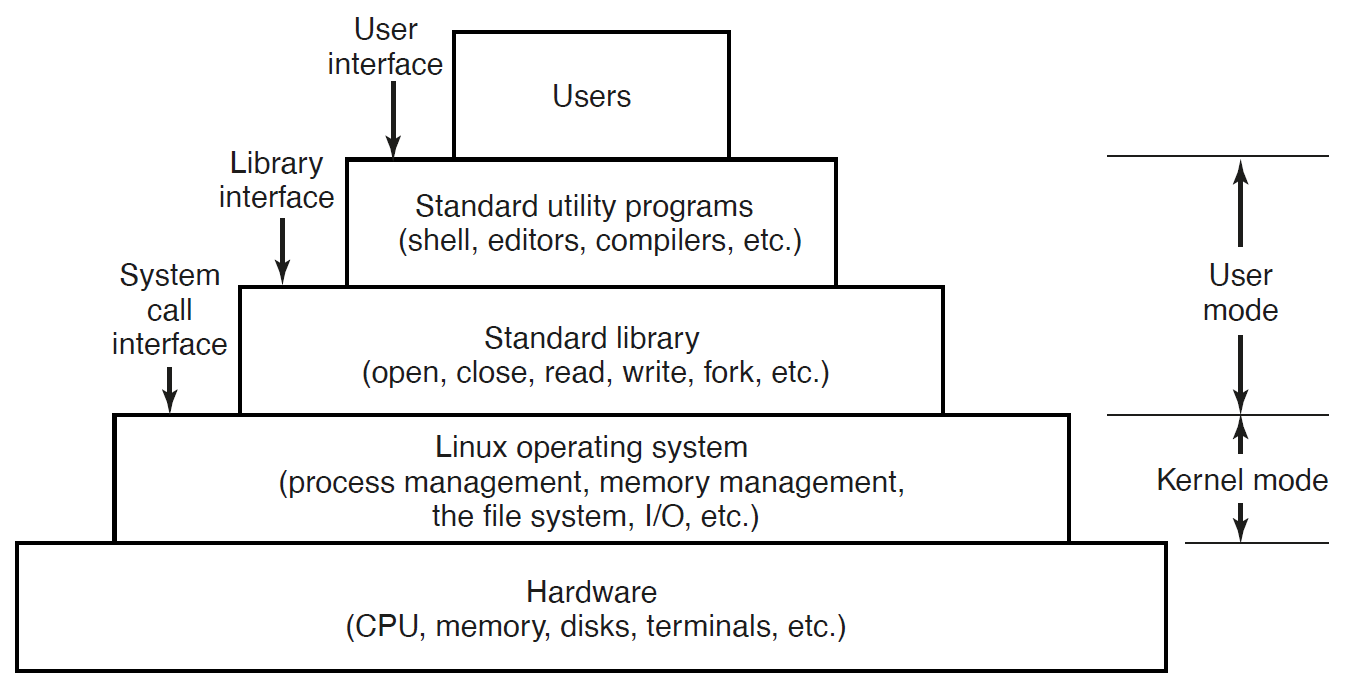
\includegraphics[width=0.9\textwidth]{images/linux_layers.png}
	\end{center}
	\caption{Linux arhitektura \cite{Tanenbaum_Bos_2023}}
	\label{fig:linux_architecture}
\end{figure}

Kar pa nas tu zares zanima, so vmesniki med posameznimi plastmi.
Predvsem nas zanima vmesnik sistemskih klicev, ki jih ponuja jedro, in vmesnik standardne knjižnice, ki nam olajša klicanje sistemskih klicev.

Standardna knjižnica nas zanima predvsem ker je uporaba vmesnika sistemskih klicev zelo odvisna od arhitekture procesorja.
Prav tako C in drugi višje nivojski programski jeziki nimajo podpore za klicanje specifičnih ukazov procesorja, ki jih potrebujemo za klicanje sistemskih klicev, to je mogoče zgolj preko zbirnega jezika \cite{Tanenbaum_Bos_2023}.
Zato bomo v nadaljevanju uporabljali standardno knjižnico, ki izpostavi preproste funkcije in poskrbi za same klice v jedro.

Ker POSIX standardi definirajo funkcije, njihove parametre, funkcionalnosti in rezultate standardne knjižnice, bo naša koda tehnično izvedljiva na katerem koli sistemu skladnem s POSIX standardom.

\subsection{Struktura jedra}

Jedro deluje direktno nad strojno opremo in ga je mogoče logično razdeliti v nekaj komponent, kot prikazuje slika \ref{fig:linux_kernel_architecture}.

\begin{figure}[h!]
	\begin{center}
		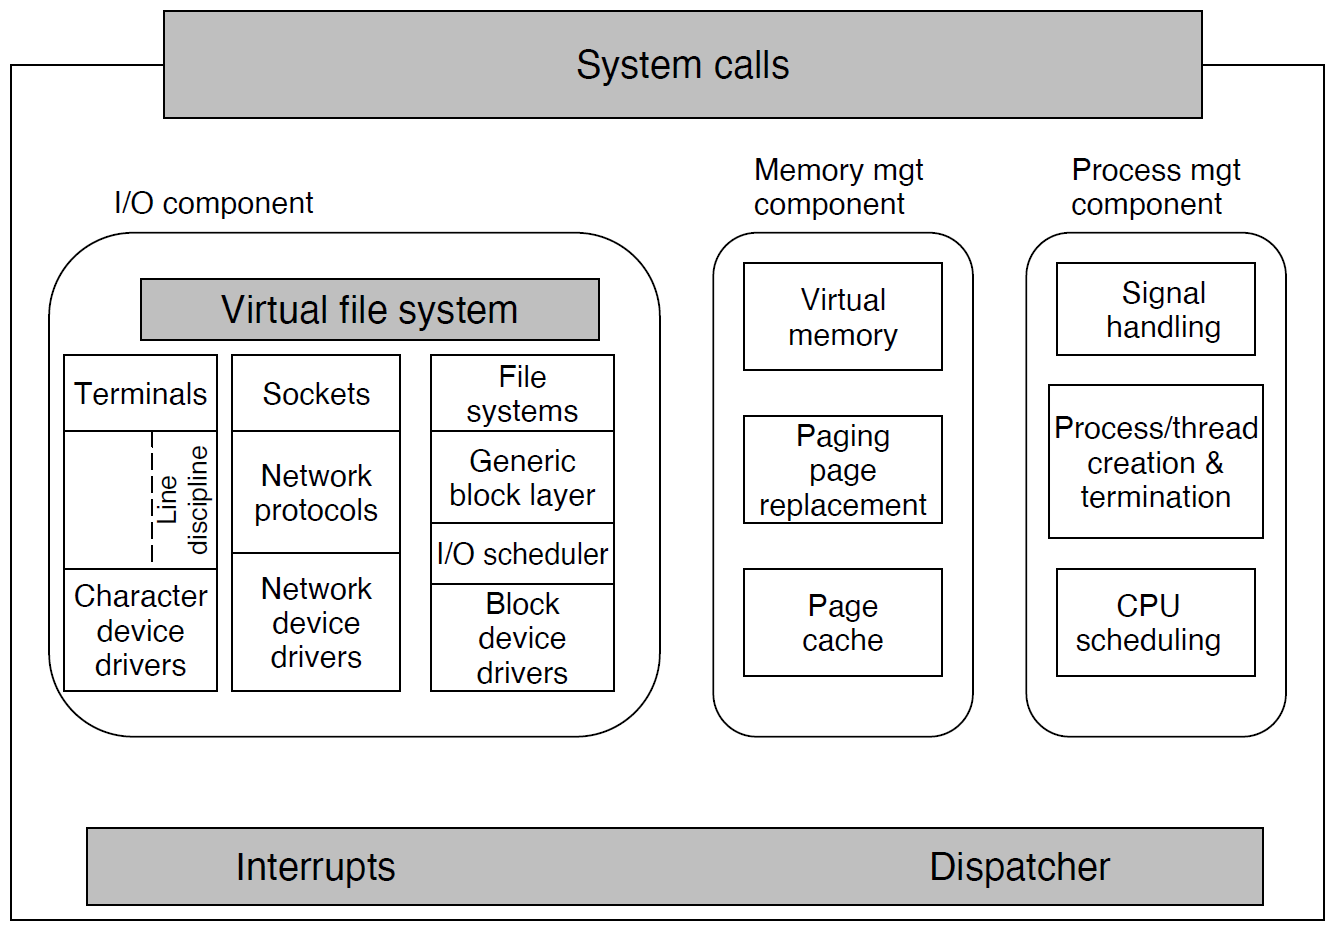
\includegraphics[width=0.9\textwidth]{images/linux_kernel_structure.png}
	\end{center}
	\caption{Linux arhitektura jedra \cite{Tanenbaum_Bos_2023}}
	\label{fig:linux_kernel_architecture}
\end{figure}

Na najnižjem nivoju jedro implementira prekinitvene rutine (\textit{angl. interrupt handler}), ki omogočajo interakcijo z napravami, 
in dodeljevalnik (\textit{angl. dispatcher}), ki upravlja procese v izvajanju in omogoča menjavanje konteksta izvajanja.

Na višjem nivoju ločujemo razne jedrne podsisteme v tri komponente.
Vhodno-izhodna komponenta vsebuje vse sisteme za interakcijo z napravami sistema \cite{Tanenbaum_Bos_2023}.
Na najvišjem nivoju komponenta združuje vse I/O operacije pod navideznim datotečnim sistemom oz. VFS (\textit{angl. Virtual File System}), ki si ga bolj podrobno pogledamo v poglavju \ref{ssec:linux:vfs}.
Na najnižjem nivoju pa se vse I/O operacije izvedejo v nekem gonilniku naprave.
Linux gonilnike klasificira kot gonilnike znakovnih naprav, ki ne omogočajo naključnega dostopa, in gonilnike bločnih naprav, ki omogočajo naključni dostop.
V diagramu so gonilniki omrežnih naprav zapisani posebej, ker so implementirani nekoliko drugače, vendar so iz tehničnega vidika klasificirani kot znakovne naprave.

Drugi dve ključni komponenti, na sliki \ref{fig:linux_kernel_architecture}, sta komponenta za upravljanje pomnilnika in komponenta za upravljanje procesov \cite{Tanenbaum_Bos_2023}.
Komponenta za upravljanje pomnilnika skrbi za povezavo virtualnega in fizičnega pomnilnika, povezane strani v pomnilniku, predpomnilnik in prenašanje novih strani v pomnilnik.
Komponenta za upravljanje procesov pa skrbi za življenjske cikle in razvrščanje procesov.
% Note: Linux obravnava tako procese kot tudi niti kot izvajalne entitete

\subsubsection{Linux Virtual File System} \label{ssec:linux:vfs}

Navidezni datotečni sistem (\textit{angl. Virtual File System -- abbr. VFS}) je programska plast v jedru, ki omogoča uporabnikom in uporabniškim programom dostop do različnih datotečnih sistemov.
Deluje pa tudi kot abstrakcija znotraj jedra, ki omogoča sobivanje različnih datotečnih sistemov.

VFS \cite{Linux_kernel_docs_LVFS} implementira vse funkcionalnosti, ki jih pričakujemo od datotečnega sistema, kot so branje in pisanje datotek, ustvarjanje in brisanje datotek, itd.
Pot do imenika, ki je podana omenjenim ukazom, se v VFS preko predpomnilnika imeniških vnosov (\textit{angl. dentry cache / dcache}) pretvori v imeniški vnos (\textit{angl. dentry}).
Ta mehanizem omogoča zelo hitro prevedbo poti v imeniški vnos, saj se izognemo branju iz diska, če seveda je imeniški vnos na voljo v predpomnilniku.

Vsak imeniški vnos vsebuje kazalec na indeksno vozlišče (\textit{angl. inode}). Indeksna vozlišča so objekti datotečnega sistema (npr. datoteke, imeniki, naprave), ki bivajo na disku (za datotečne sisteme blokovnih naprav) ali v pomnilniku (za pseudo datotečne sisteme).
Indeksna vozlišča, ki bivajo na disku se, po potrebi, kopirajo v pomnilnik, spremembe pa se zapišejo nazaj na disk.
Eno indeksno vozlišče lahko pripada več imeniškim vnosom, kar omogoča, da se datoteka prikaže na več različnih mestih v imeniku.

VFS omogoča UNIX koncept ``everything is a file'', kjer je osnovna ideja, da se vsi sistemski resursi (npr. naprave, procesi, omrežje) predstavijo kot datoteke.
To omogoča enoten način dostopa do sistemskih virov, kar olajša uporabo in razvoj programske opreme in zmanjša število potrebnih sistemskih klicev.

\section{Operacijski sistem Windows}

Windows je zaprtokodni operacijski sistem, ki ga razvija Microsoft.
Nastopa v več različnih družinah, vsaka s svojo ciljno publiko od uporabniških računalnikov in strežnikov do IoT in vgrajenih sistemov.

Danes je Windows najbolj popularen operacijski sistem za namizne računalnike, s približno 70\% tržnim deležem.

\subsection{Zgodovina}

Razvoj Windows se je začel leta 1988 pod okriljem Microsoft in IBM.
Cilj je bil razviti NT (\textit{``New Technology''}) operacijski sistem s podporo za OS/2 in POSIX aplikacijska vmesnika, vendar je tekom razvoja nastal ločen 32-bitni Windows aplikacijski vmesnik pod imenom Win32.

V NT verziji 4.0, ki se je uporabljala v Windows 95, je jedro vsebovalo spletni strežnik in brskalnik, skupaj z vso grafično logiko in uporabniškim vmesnikom.
Te spremembe so bile uvedene z namenom izboljšanja učinkovitosti, stranski učinek pa je bila zmanjšana zanesljivost sistema.

V Windows 2000 so dodali podporo za Active Directory, ``plug-and-play'' naprave in porazdeljen datotečni sistem.
Prav tako so izboljšali omrežno podporo ter podprli več različnih procesorjev, vendar samo Intel (in kompatibilne) procesorje, in več sistemskega pomnilnika.

Naslednji večji skok v razvoju je bil Windows XP, ki je na trg nastopil z prenovljenim grafičnim okoljem in samodejnim odpravljanjem težav z aplikacijami in samim operacijskim sistemom.
S temi spremembami je Windows XP zagotavljal boljše omrežne storitve, podporo za več naprav ter ogromno izboljšavo v zmogljivosti, zanesljivosti in varnosti.
Prav tako je bila prva izdaja s podporo za 64-bitne sisteme.

Leta 2006 je bil izdan Windows Vista, ki kljub mnogim izboljšavam, zaradi težav z nekompatibilnostmi in počasnim odzivnim časom, ni požel velikega uspeha.
Med najbolj ključnimi izboljšavami je bil premik grafične implementacije v ``desktop window manager'', ki se je izvajal kot uporabniški proces.

Naslednji večji skok je nastopil z Windows 7, ki je bil izdan leta 2009, in je odpravil večino težav svojega predhodnika.
% TODO: Win 8, 10, 11
%\cite{Silberschatz_Galvin_Gagne_2018}

Glavna cilji pri razvoju Windows NT so bila \cite{Yosifovich_Russinovich_Solomon_Ionescu_2017}:
\begin{itemize}
	\item Razširljivost
	      \begin{description}
	      	\item Koda mora biti napisana tako, da lahko brez težav raste in prilagodi zahtevam na trgu.
	      \end{description}
	\item Prenosnost
	      \begin{description}
	      	\item Sistem se mora izvajati na različnih arhitekturah in ohranjati možnost prehoda na nove arhitekture.
	      \end{description}
	\item Zanesljivost in robustnost
	      \begin{description}
	      	\item Sistem se mora zaščititi pred internimi napakami in zunanjimi vplivi. Aplikacije ne morejo škodovati OS ali drugim aplikacijam.
	      \end{description}
	\item Kompatibilnost
	      \begin{description}
	      	\item Kljub temu, da Windows NT razširja funkcionalnosti obstoječih tehnologij, naj bodo programski vmesniki kompatibilni s starejšimi verzijami Windows in MS-DOS. Prav tako naj dobro sodeluje z drugimi sistemi kot UNIX, OS/2 ub NetWare.
	      \end{description}
	\item Zmogljivost
	      \begin{description}
	      	\item Upoštevajoč druge zahteve, naj bo sistem kar se da zmogljiv in hiter na vsaki platformi.
	      \end{description}
\end{itemize}

Seveda so se te cilji spreminjali tekom razvoja.

\subsection{Arhitektura}

Windows je monoliten operacijski sistem, v smislu da si večina kode OS in gonilnikov deli isti privilegiran naslovni prostor \cite{Yosifovich_Russinovich_Solomon_Ionescu_2017}.
To pomeni, da lahko katera koli komponenta OS ali gonilnik potencialno okvari/spremeni podatke, ki jih uporabljajo druge komponente OS.

V poskusu zmanjšanja verjetnosti tovrstnih napak, Windows zahteva digitalno podpisane gonilnike.
Gonilnik mora najprej z ustreznim certifikatom podpisati izdajatelj, ter ga oddati v pregled na Microsoftov portal.
Ko Microsoft potrdi delovanje gonilnika, ga podpiše še s svojim digitalnim certifikatom in šele nato bo operacijski sistem sprejel in izvajal gonilnik.

\begin{figure}[h!]
	\begin{center}
		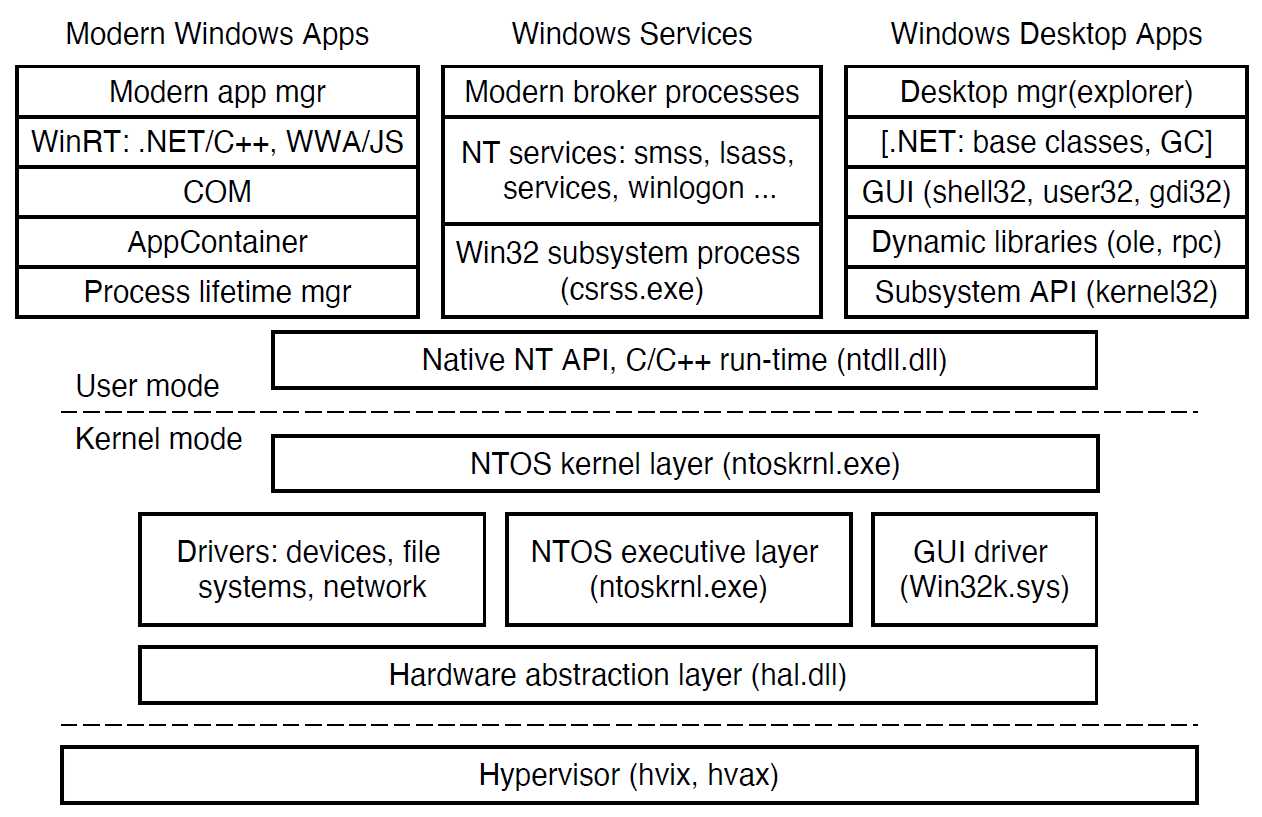
\includegraphics[width=\textwidth]{images/windows_programming_layers.png}
	\end{center}
	\caption{Windows arhitektura \cite{Tanenbaum_Bos_2023}}
	\label{fig:windows_architecture}
\end{figure}

Jedro NT operacijskega sistema je NTOS jedrni program (\textit{ntoskrnl.exe}), ki izpostavlja vmesnik sistemskih klicev.
Vmesnik sistemskih klicev in uporabniška knjižnica (\textit{ntdll.dll}) sta v celoti delo Microsoft programerjev in v večjem delu nedokumentirana.
Uporabniški vmesniki so del osebnosti operacijskega sistema, ki se imenujejo podsistemi (\textit{angl. subsystem}).

Originalno je NT podpiral tri podsisteme: Win32, POSIX in OS/2.
Podpora za OS/2 je bila odstranjena v izdaji Windows XP, podpora za POSIX pa v Windows 8.1.
Danes so vse Windows aplikacije napisane z uporabo Win32 API, ki ga izpostavlja Win32 podsistem.
Microsoft, preko Github projekta \href{https://github.com/microsoft/win32metadata}{microsoft/win32metadata}, objavlja opis celotne Win32 API površine v standardiziranem formatu (ECMA-335) na tak način, da omogoča izgradnjo projekcij v več programskih jezikov.
To omogoča pisanje Windows aplikacij tako v privzetem C/C++ kot tudi v drugih jezikih.

\subsection{Windows Podsistemi}

Kot prikazuje slika \ref{fig:windows_subsystems_components}, so NT podsistemi sestavljeni iz štirih komponent: procesa podsistema, nabora knjižnic, sistemskih kljuk in podpora v jedru \cite{Tanenbaum_Bos_2023}.
Proces podsistema je storitev, ki jo zažene upravljalnik sej (\textit{smss.exe}) -- prvi uporabniški proces, ki se zažene v Windows.

Kljub temu, da je Win32 sedaj edini podprti podsistem, se Windows drži modela podsistemov za potencialne prihodnje razširitve.

\begin{figure}[h!]
	\begin{center}
		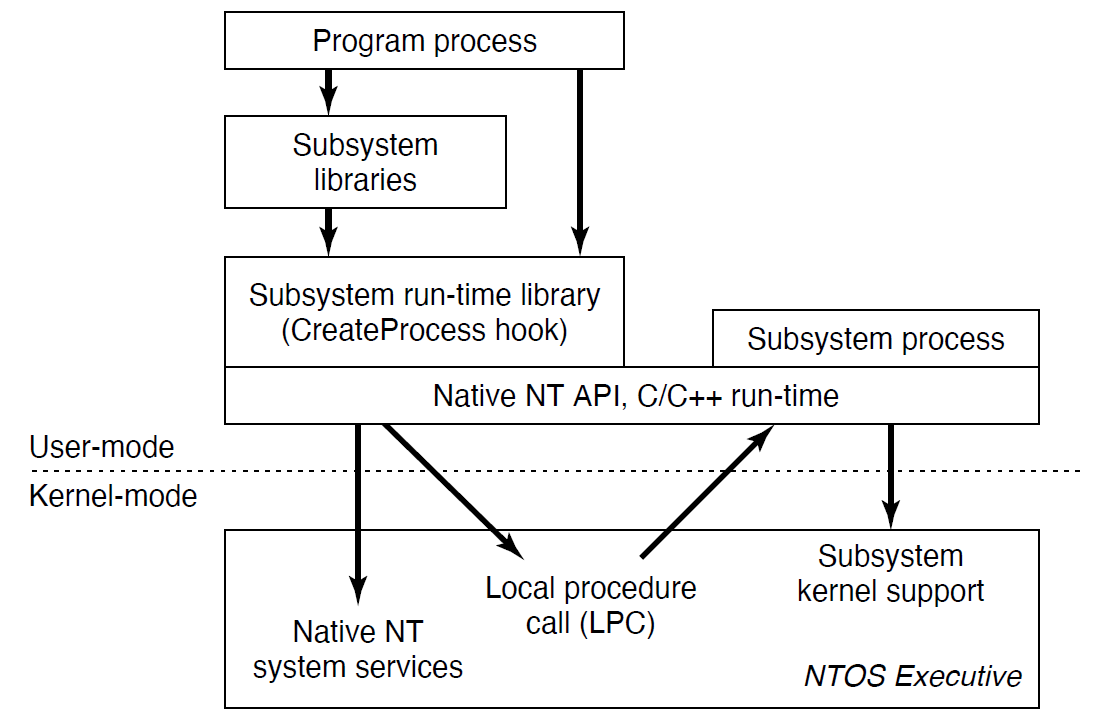
\includegraphics[width=0.9\textwidth]{images/windows_subsystems_components.png}
	\end{center}
	\caption{Komponente Windows podsistemov \cite{Tanenbaum_Bos_2023}}
	\label{fig:windows_subsystems_components}
\end{figure}

\subsubsection{Win32 podsistem}

Win32 funkcijski klici se kolektivno imenujejo Win32 API.
To so polno dokumentirani javno objavljeni vmesniki, implementirani kot procedure, ki kličejo NT sistemske klice ali, v nekaterih primerih, opravijo delo v uporabniškem načinu \cite{Tanenbaum_Bos_2023}.
Za ohranjanje aplikacijske kompatibilnosti se obstoječi Win32 API klici ne spreminjajo z novimi izdajami Windows, se pa dodajajo nove funkcije.

Programi napisani za starejše verzije Win32, bi teoretično morale delovati v novejših verzijah sistema, saj se je Win32 API zelo malo spreminjal.
V imenu kompatibilnosti Windows podpira dva posebna izvajalna okolja imenovana WoW oz. Windows-on-Windows.
WoW32 se uporablja na 32-bitnih x86 sistemih za izvajanje 16-bitnih Windows aplikacij. Zadnja izdaja sistema, ki podpira WoW32 je bil Windows 10.
WoW64 pa omogoča izvajanje 32-bitnih aplikacij na 64-bitnem sistemu.
V Windows 10 je bila ta funkcionalnost še razširjena za izvajanje 32-bitnih x86 aplikacij na arm64 sistemih.
V Windows 11 pa ta emulacija podpira tudi izvajanje 64-bitnih x86-64 aplikacij na arm64 sistemih.

Osnovna filozofija Win32 se precej razlikuje od UNIX pristopa.
V UNIX sistemih so funkcije OS precej preproste, z malo parametri in redko najdemo več kot en način za izvedbo določene operacije.
Win32 pa zagotavlja obsežen nabor vmesnikov, z veliko parametri in običajno najdemo tri ali štiri načine za izvedbo določene operacije.
Pogosto vidimo tudi mešanje nizko in visoko nivojskih funkcij v istem vmesniku.
To pomeni, da Win32 zagotavlja funkcionalno zelo bogat nabor vmesnikov, vendar vnese veliko kompleksnosti zaradi slabše strukture vmesnikov, ki mešajo nizko in visoko nivojske funkcije v isti API \cite{Tanenbaum_Bos_2023}.

\subsection{Windows Register}

Ob zagonu sistema Windows ustvari NT imenski prostor, na katerega se pripenjajo datotečni volumni.
To pomeni, da mora sistem nekje drugje pridobiti konfiguracijo potrebno ob zagonu.
V ta namen se uporablja poseben datotečni sistem, ki se pripne na NT imenski prostor.
Ta datotečni sistem se imenuje register (\textit{angl. registry}) in je optimiziran za majhne datoteke \cite{Tanenbaum_Bos_2023}.

Register je organiziran v ločene volumne, ki jih imenujemo gnezda (\textit{angl. hive}).
Vsako gnezdo se hrani v svoji datoteki v imeniku \texttt{C:\symbol{92}Windows\symbol{92}system32\symbol{92}config\symbol{92}} na zagonskem volumnu.

Ob zagonu sistema se gnezdo \texttt{SYSTEM} naloži v pomnilnik.
V njem se hranijo ključne informacije kot gonilniki, zagonski programi in drugi parametri za inicializacijo sistema.

Poleg tega ima Windows še druga gnezda kot vidimo v tabeli \ref{tab:windows_registry_hives}.

\begin{table}[h!]
	\begin{center}
		\begin{tabular}{ p{3.7cm}|p{8.8cm} }
			Gnezdo     & Namen                                         \\
			\hline
			SYSTEM     & OS konfiguracija                              \\
			HARDWARE   & zapisi o zaznani strojni opremi               \\
			BCD        & baza za konfiguracijo obuvanja                \\
			SAM        & informacije o lokalnih uporabniških računih \\
			SECURITY   & informacij o zaščiti                        \\
			DEFAULT    & privzeto gnezdo za nove uporabnike            \\
			NTUSER.DAT & gnezdo uporabnika, v domačem imeniku         \\
			SOFTWARE   & aplikacijski razredi COM                      \\
			COMPONENTS & manifesti in odvisnosti sistemskih komponent  \\
		\end{tabular}
	\end{center}
	\caption{Gnezda Windows registrov \cite{Tanenbaum_Bos_2023}}
	\label{tab:windows_registry_hives}
\end{table}

\section{Sistemski klici} \label{sec:syscalls}

Sistemski klici so vmesnik do storitev, ki jih ponuja jedro operacijskega sistema, kot na primer ustvarjanje procesov, branje in pisanje datotek, komunikacijo med procesi, itd.
Ker torej sistemski klici prehajajo med uporabniškim in jedrnim načinom procesorja (več o tem v poglavju \ref{sec:syscall_execution}), je njihova implementacija odvisna od arhitekture procesorja in njegovega nabora ukazov.

Ker pa jih uporabniški programi potrebujejo dokaj pogosto, so v večini operacijskih sistemov izpostavljeni preko knjižnice ali API-ja.
Najbolj pogosto uporabljena API-ja za aplikacijske programerje sta \textbf{POSIX}, za sisteme ki sledijo POSIX standardu (npr. Unix, Linux in macOS), in \textbf{Windows API}, za Windows sisteme.
Programer do API dostopa preko knjižnice, ki jo ponuja operacijski sistem -- npr. glibc za programski jezik C, v primeru Linuxa.
Tu je omembe vredno tudi, da imena funkcij v knjižnici niso nujno enaka imenom sistemskih klicev, ki jih uporablja sistem.

Ker je sistemskih klicev ogromno, jih bomo v nadaljevanju razdelili na šest kategorij \cite{Silberschatz_Galvin_Gagne_2018}, in sicer:
\begin{itemize}
	\item \textbf{upravljanje procesov}
	      \begin{description}
	      	\item kreiranje in ustavljanje procesov, nalaganje in izvajanje programa, upravljanje atributov procesa, sprejemanje in oddajanje signalov, zasedanje in sproščanje pomnilnika
	      \end{description}
	\item \textbf{upravljanje datotek}
	      \begin{description}
	      	\item kreiranje, brisanje, odpiranje in zapiranje datotek, branje in pisanje, premikanje datotek, upravljanje atributov datotek
	      \end{description}
	\item \textbf{upravljanje naprav}
	      \begin{description}
	      	\item zahtevanje in sproščanje naprav, branje in pisanje v napravo, upravljanje atributov naprav, logično pripenjanje in odpenjanje naprav
	      \end{description}
	\item \textbf{vzdrževanje informacij o sistemu}
	      \begin{description}
	      	\item upravljanje sistemskega časa, upravljanje informacij sistema, pridobivanje in nastavljanje atributov procesov, datotek in naprav
	      \end{description}
	\item \textbf{komunikacija med procesi}
	      \begin{description}
	      	\item kreiranje in brisanje komunikacijskih kanalov, pošiljanje in sprejemanje sporočil, prenos informacij o statusu, pripenjanje in odpenjanje oddaljenih naprav
	      \end{description}
	\item \textbf{zaščita}
	      \begin{description}
	      	\item upravljanje pravic procesov, datotek in naprav
	      \end{description}
\end{itemize}

% Preden pa se podamo v primerjave posameznih sistemskih klicev, si poglejmo še, kakšne so implementacijske razlike med sistemskimi klici v Linuxu in Windowsu.
% Tu še enkrat poudarjam, da so razlike med sistemskimi klici odvisne od arhitekture procesorja.
% V vseh konkretnih primerih bom uporabljal ukazni nabor in imena registrov arhitekture \textbf{x86}.

\section{Izvedba sistemskega klica} \label{sec:syscall_execution}

Kot smo že povedali, imajo operacijski sistemi dve glavni funkciji: upravljanje sistemskih virov in zagotavljanje abstrakcij za uporabniške aplikacije.
Upravljanje virov je v večini primerov transparentno uporabnikom in se izvaja v ozadju. Zato je vmesnik med programi in operacijskim sistemom predvsem osredotočen na abstrakcije sistema \cite{Tanenbaum_Bos_2023}.
Da lahko res razumemo kaj operacijski sistemi počnejo, si moramo pobližje pogledati ta vmesnik.

Moderne procesorske arhitekture definirajo več privilegijskih nivojev ali obročev.
Vzemimo za primer arhitekturo x86 \cite{Intel_2024}, ki implementira 4 nivoje oz. obroče (številčene od 0 do 3) kot prikazuje slika \ref{fig:privilege_levels_x86}.
Večja številka pomeni manj privilegijev.
Srednji obroč oz. nivo 0 se uporablja za najbolj kritično programsko opremo, običajno jedro operacijskega sistema.
Zunanji obroči oz. nivoji 1 do 3 pa se uporabljajo za manj kritično programsko opremo.
Kako operacijski sistem koristi nivoje izvajanja je odvisno od implementacije.
Sistemi, ki uporabljajo samo dva nivoja izvajanja, uporabljajo nivo 0 za jedro in nivo 3 za uporabniške programe.

Procesor uporabi nivoje, da zaščiti segmente bolj privilegiranih procesov pred manj privilegiranimi.
Prav tako ima procesor poseben nabor navodil, ki se imenujejo privilegirana navodila.
Le-ta se lahko uporabljajo samo v nivoju 0.

Kadar procesor zazna kršitev nivoja, sproži izjemo in tako obvesti jedro o napaki.

\begin{figure}[h!]
	\begin{center}
		\begin{tikzpicture}
			\draw (0, 0) circle (1);
			\draw (0, 0) circle (2);
			\draw (0, 0) circle (3);
			\draw (0, 0) circle (4);
			\node [align=right] at (-6.5, -1.5) {
				\shortstack[r]{\small{Operating}\\\small{System}\\\small{Kernel}}\\\\
				\shortstack[r]{\small{Operating System}\\\small{Services}}\\\\
				\small{Applications}
			};
			\node at (0, -.2) {Level 0};
			\node at (0, -1.5) {Level 1};
			\node at (0, -2.5) {Level 2};
			\node at (0, -3.5) {Level 3};
			\draw[->] (-4.5, .3) -- (0, .3);
			\draw[->] (-4.5, -1.7) -- (0, -1.2);
			\draw[->] (-4.5, -1.7) -- (0, -2.2);
			\draw[->] (-4.5, -3.2) -- (0, -3.2);
		\end{tikzpicture}
	\end{center}
	\caption{Nivoji zaščite v x86 arhitekturi \cite{Intel_2024}}
	\label{fig:privilege_levels_x86}
\end{figure}

Ker pa je število nivojev in njihov namen drugačen od arhitekture do arhitekture, jih posplošimo dva nivoja delovanja: \textbf{uporabniški} in \textbf{jedrni} oz. privilegiran način.
Kot že omenjeno, se jedro operacijskega sistema izvaja v jedrnem načinu, kjer ima dostop do vseh virov sistema in lahko izvede kateri koli ukaz v ukaznem naboru procesorja.
Preostanek programske opreme pa se izvaja v uporabniškem načinu, kjer ima omejen dostop.

Ker je način izvedbe klica odvisen od arhitekture sistema in običajno zahteva implementacijo v zbirnem jeziku, večina operacijskih sistemov zagotavlja knjižnico v višje-nivojskem jeziku -- običajno C ali C++.
Kljub temu, da iz uporabniške oz. programske strani sistemski klici v knjižnici izgledajo kot običajne funkcije, pa je njihova implementacija popolnoma drugačna \cite{Tanenbaum_Bos_2023}:
\begin{enumerate}
	\item Uporabniški proces (oz. knjižnica, ki jo uporablja) shrani številko sistemskega klica in argumente funkcije v registre procesorja -- registri se razlikujejo glede na arhitekturo in OS.
	\item Uporabniški proces proži past, ki preklopi procesor v jedrni način in požene prekinitveni servisni program (ISR), ki ga je definiral operacijski sistem.
	\item Jedro izvede zahtevan sistemski klic kot katero koli drugo funkcijo in vrne rezultat -- rezultat se zapiše v register iz katerega ga uporabniški program lahko prebere.
	\item Procesor preklopi nazaj v uporabniški način in nadaljuje izvajanje uporabniškega procesa.
\end{enumerate}

\section{Programski vmesnik Linux -- POSIX API}

Linux API je implementiran preko glibc oz. GNU C knjižnice, ki zagotavlja API vmesnik po standardih ISO C11, POSIX.1-2008 in BSD ter druge OS-specifične API vmesnike \cite{GNU_Manual}.
Prav tako je kompatibilna s starejšimi verzijami ISO C.
Celotna GNU C knjižnica je odprtokodna pod licenčnimi pogoji LGPL 2.1.

Ker pa je Linux jedro odprtokodno pod licenco GPL 2.0, si lahko pogledamo tudi celotno implementacijo jedra.
Za nas je najbolj relevantna tabela sistemskih klicev.
Ta je, za x86 64-bitno arhitekturo dostopna v datoteki \texttt{arch/x86} \texttt{/entry/syscalls/syscall\_64.tbl} v \href{https://github.com/torvalds/linux}{izvorni kodi jedra}.
Tu lahko opazimo, da je arhitektura procesorja del poti do datoteke in če pogledamo v druge imenike v \texttt{arch}, lahko vidimo, da ima vsaka implementirana arhitektura med drugim tudi svojo tabelo sistemskih klicev.

Kot smo že povedali Linux sledi standardu POSIX, ki definira procedure aplikacijskega vmesnika.
V veliki večini te procedure zahtevajo uporabo sistemskih klicev, vendar je potrebno poudariti, da povezava ni nujno ena proti ena.
Lahko se zgodi, da je neka procedure izvedljiva v uporabniškem načinu in ne zahteva sistemskega klica, ali pa zahteva uporabo več sistemskih klicev.
V nekaterih primerih se lahko zgodi tudi, da več procedur uporablja isti (bolj splošen) sistemski klic.
Te specifike si bomo pobližje ogledali v naslednjem poglavju.

\section{Programski vmesnik Windows -- Windows API}

Windows je, v kontrastu z Linuxom, zaprtokodni operacijski sistem, zato je težje najti dokumentacijo o njegovi implementaciji.
Ena izmed glavnih razlik je, da Windows omogoča dostop do sistemskih klicev izključno preko Windows API-ja.
Torej, če smo v Linuxu lahko pokukali v tabelo sistemskih klicev in jih lahko celo poklicali direktno z zbirnim jezikom, je v Windowsu to nemogoče.

Še ena velika razlika, ki jo bomo srečavali v naslednjem poglavju, je število API procedur.
Windows API izpostavi ogromno procedur, v rangu več tisoč, medtem ko POSIX API izpostavi le nekaj sto \cite{Tanenbaum_Bos_2023}.
To je posledica več faktorjev -- pogosto več funkcij uporablja isti sistemski klic, veliko pa je tudi funkcij, ki so v celoti implementirane v uporabniškem načinu.

Ker Windows ne izpostavi sistemskih klicev direktno, se lahko le-te spreminjajo med posameznimi verzijami operacijskega sistema \cite{Tanenbaum_Bos_2023}.
To pomeni, da je težko zagotovo reči ali je neka funkcija implementirana v jedru ali uporabniški knjižnici.

Windows se od večine operacijskih sistemov razlikuje po kodiranju internih znakovnih nizov \cite{Yosifovich_Russinovich_Solomon_Ionescu_2017}. Uporablja namreč 13-bitno Unicode kodiranje.
Ker pa mnogo aplikacij uporablja 8-bitno ANSI kodiranje, ima večina Windows funkcij dve verziji: tako, ki sprejema ANSI znake in tako, ki sprejema 16-bitne Unicode znake.
8-bitne verzije funkcij so posledično rahlo počasnejše, saj se niz najprej pretvori v Unicode.

\begin{table}[h!]
	\begin{center}
		\begin{tabular}{ l|l }
			Win32 API klic         & NT API klic                 \\
			\hline
			\verb|CreateProcess|   & \verb|NtCreateProcess|      \\
			\verb|CreateThread|    & \verb|NtCreateThread|       \\
			\verb|ReadFile|        & \verb|NtReadFile|           \\
			\verb|DeleteFile|      & \verb|NtSetInformationFile| \\
			\verb|DuplicateHandle| & \verb|NtDuplicateObject|    \\
			\verb|CloseHandle|     & \verb|NtClose|              \\
		\end{tabular}
	\end{center}
	\caption{Primeri Win32 API klicev vezanih NT API klicev \cite{Tanenbaum_Bos_2023}}
	\label{tab:example_win32_nt_mapping}
\end{table}

V tabeli \ref{tab:example_win32_nt_mapping} si pogledamo nekaj primerov Win32 API klicev in NT API klicev, ki jih kličejo.
Zanimivo je da so povezave tako nezanimive.
Večina nizko nivojskih Win32 funkcij ima direktne NT ekvivalente kar ni preveč presenetljivo, saj je bil Win32 oblikovan z NT v mislih\cite{Tanenbaum_Bos_2023}.
Pogosto Win32 funkcije samo manipulirajo parametre in kličejo NT funkcije.
Nekateri Win32 klici sprejmejo pot do objekta medtem ko NT ekvivalentna funkcija pričakuje ročico objekta (\textit{angl. handle}).
Prav tako je naloga Win32 API klicev, da pretvorijo znakovne nize iz ANSI v Unicode kodiranje.

TODO: Nedokumentiran del API-ja (Ntoskrnl.exe, Win32k.sys, ntdll.dll) pg. 49, Ne-strukturirano procesno drevo

\chapter{Procesi}

Proces je program (strojna koda) v izvajanju, katerega status predstavljajo programski števec in vsebina procesorskih registrov.
Proces ima tudi svoj prostor v pomnilniku, ki je običajno razdeljen na več segmentov:
\begin{itemize}
	\item \textbf{podatkovni} (\textit{angl. data}) -- vsebuje vrednosti globalnih spremenljivk,
	\item \textbf{programski} (\textit{angl. text}) -- vsebuje strojno kodo programa,
	\item \textbf{sklad} (\textit{angl. stack}) -- vsebuje vrednosti lokalnih spremenljivk in povratne naslove funkcij in
	\item \textbf{kopica} (\textit{angl. heap}) -- dinamično dodeljen pomnilnik \cite{Silberschatz_Galvin_Gagne_2018}.
\end{itemize}

\begin{figure}[h!]
	\begin{center}
		\begin{tikzpicture}
			\filldraw[fill=blue!20!white] (0, 0) rectangle (4, 8);
			\draw node at (-1, 0) {0};
			\draw node at (-1, 8) {max};
			\filldraw[fill=gray!40!white] (0, 8) rectangle (4, 6.5) node[pos=.5] {stack};
			\draw[arrow] (2, 6.5) -- (2, 5.8);
			\draw[arrow] (2, 3.5) -- (2, 4.2);
			\filldraw[fill=gray!40!white] (0, 2) rectangle (4, 3.5) node[pos=.5] {heap};
			\filldraw[fill=gray!40!white] (0, 1) rectangle (4, 2) node[pos=.5] {data};
			\filldraw[fill=gray!40!white] (0, 0) rectangle (4, 1) node[pos=.5] {text};
		\end{tikzpicture}
	\end{center}
	\caption{Segmenti pomnilnika procesa}
\end{figure}

\section{Pregled funkcionalnosti}

Sistemski klici za procesni nadzor skrbijo za:
\begin{itemize}
	\item ustvarjanje in končanje procesov,
	\item nalaganje in izvajanje programov,
	\item pridobivanje in nastavljanje atributov procesov,
	\item sinhronizacijo procesov,
	\item dodeljevanje in sproščanje pomnilnika \cite{Silberschatz_Galvin_Gagne_2018}.
\end{itemize}

\section{Sistemski klici v Linux}

\subsection{Ustvarjanje in končanje procesa}

\subsubsection{\texttt{fork}}

\texttt{pid_t fork(void);}

Funkcija \texttt{fork()} ustvari nov proces, ki je fuplikat izvajajočega procesa.
Nov proces postane otrok klicajočega procesa.

Otroški proces je identična kopija starševskega, z izjemo nekaj ključnih točk:
\begin{itemize}
	\item Identifikator procesa (PID) je unikaten za vsak proces, otrok torej dobi nov PID.
	\item Identifikator starševskega procesa (PPID) postane enak kot PID starševskega (klicajočega) procesa.
	\item Otrok ne deduje starševih pomnilniških ključavnic.
	\item Ponastavijo se števci uporabe virov in CPU časa.
	\item Otrok ne deduje čakajočih signalov.
	\item Otrok ne deduje datotečnih ključavnic asociiranih s procesov. Deduje pa ključavnice asociirane z odprtimi datotekami.
	\item Otrok ne deduje obstoječih asinhronih I/O operacij ali asinhronih I/O kontekstov.
\end{itemize}

Funkcija ne sprejme nobenih vhodnih parametrov, vrne pa \texttt{0} v otroškem procesu in PID otroškega procesa v starševskem procesu.
V primeru napake funkcija vrne \texttt{-1} starševsskemu procesu in ne ustvari otroškega procesa.

Vredno je pripomniti, da je \texttt{fork} v Linux implementiran preko tako imenovanega ``copy-on-write'' mehanizma.
To pomeni, da kreiranje novega procesa zahteva minimalno kopiranje v pomnilniku, saj se to izvede šele ko je re potrebno -- tj. ko proces začne spreminjati pomnilnik.

\subsubsection{\texttt{execve}}

\texttt{int execve(const char *pathname, char *const _Nullable argv[],
char *const _Nullable envp[]);}

Ko želimo zagnati nov proces, ki izvaja drug program, takoj za klicem \texttt{fork} kličemo funkcijo \texttt{execve()}.
\texttt{execve()} zamenja programski spomin trenutnega procesa z programom v podani datoteki.
Prav tako na novo inicializira sklad, kopico in odatkovne segmente.

Če ima program (datoteka), ki ga nalagamo, nastavljen ``setuid'' bit, se efektivni uporabniški ID procesa spremeni na ID lastnika datoteke.
Enako se zgodi če ima program nastavljen ``getgid'' bit, samo da se ta navezuje na ID skupine.
Te pravili pa imata nekaj izjem, ki se navezujejo na atribute klicajoče niti.

\texttt{execve} ohrani vse atribute procesa z nekaj izjemami:
\begin{itemize}
	\item Dispozicije (akcije) signalov se ponastavijo.
	\item Preslikani pomilniki se ne ohranijo.
	\item Regije deljenega pomnilnika, vrste, semaforji, časovniki in ključavnice se ne ohranijo.
	\item Vse niti razen kicajoče so usstavljene.
\end{itemize}

Funkcija sprejme tri argumente: pot do programa, argumente programa (opcijski) in okoljske spremenljivke programa (opcijski).
Ob uspešni izvedbi funkcija ne vrne ničesar, saj se začne izvajati novo naloženi program, v primeru napake pa vrne \texttt{-1}.

\subsubsection{\texttt{exit}}

\texttt{void exit(int status);}

Ko želimo trenutni proces ustaviti, pokličemo funkcijo \texttt{exit()}, ki zaključi in uniči proces.
Sistem zapre odprte dokumente, osirotene (otroške) procese podeduje začetni proces (PID 1) in staršu pošlje signal SIGCHLD.

Funkcija sprejme argument \textit{status}, katerega spodnji oktet oz. bajt je posredovan staršu.
Funkcija v nobenem primeru ne vrne ničesar, saj se proces zaključi.

Več o signalu SIGCHLD in posredovanju statusa staršu v poglavju \ref{ssec:linux_syscalls:waiting}.

\subsubsection{\texttt{kill}}

\subsection{Čakanje} \label{ssec:linux_syscalls:waiting}

\subsection{Niti}

\subsection{Spanje}

\subsection{Pridobivanje sistemskih informacij}

\section{Sistemski klici v Windows}

\subsection{Ustvarjanje in končanje procesa}

\subsection{Čakanje}

\subsection{Niti}

\subsection{Spanje}

\subsection{Pridobivanje sistemskih informacij}

\section{Primerjava sistemov}

\chapter{Upravljanje procesov} \label{sec:process_control}

\section{Primerjava sistemskih klicev}

\begin{table}[h!]
	\begin{center}
		\begin{tabular}{ p{3.7cm}|p{2.5cm}|p{6cm} }
			Function          & Linux                                                  & Windows                                                                                                                                                                         \\
			\hline
			Ustvari proces    & \verb|fork|\newline\verb|vfork|                        & \verb|CreateProcess|\newline\verb|CreateProcessAsUser|\newline\verb|CreateProcessWithLogonW|\newline\verb|CreateProcessWithTokenW|                                              \\
			Ustavi proces     & \verb|exit|                                            & \verb|ExitProcess|                                                                                                                                                              \\
			Ubij proces       & \verb|kill|                                            & \verb|TerminateProcess|                                                                                                                                                         \\
			Naloži program   & \verb|execve|                                          & \textit{naloženo pri ustvarjanju}                                                                                                                                              \\
			Sinhronizacija    & \verb|wait|\newline\verb|waitpid|\newline\verb|waitid| & \verb|WaitForSingleObject|\newline\verb|WaitForMultipleObjects|                                                                                                                 \\
			Ustvari nit       & \verb|clone|                                           & \verb|CreateThread|                                                                                                                                                             \\
			Ubij nit          & \verb|kill|                                            & \verb|TerminateThread|                                                                                                                                                          \\
			Počakaj          & \verb|nanosleep|                                       & \verb|Sleep|                                                                                                                                                                    \\
			Pridobivanje info & \verb|getpid|\newline\verb|getppid|                    & \verb|GetCurrentProcess|\newline\verb|GetCurrentProcessId|\newline\verb|GetCommandLine|\newline\verb|GetCurrentProcessorNumber|\newline\verb|GetEnvironmentVariable|\newline... \\
		\end{tabular}
	\end{center}
	\caption{Povzetek sistemskih klicev za procesni nadzor}
	\label{tab:process_control}
\end{table}

V tabeli \ref{tab:process_control} vidimo, da je velik del sistemskih klicev za procesni nadzor simetričen med obema operacijskima sistemoma.
Opazimo pa, da Windows ne ponuja sistemskih klicev za nalaganje programov, saj se to zgodi ob ustvarjanju procesa, medtem ko Linux ustvari nov proces s kloniranjem trenutnega procesa in nato omogoča nalaganje drugega programa.
Prav tako opazimo, da Windows ponuja več sistemskih klicev za pridobivanje informacij o procesu, Linux pa te informacije hrani v virtualnem datotečnem sistemu in te informacije za dan proces pridobivamo iz datotek v imeniku \verb|/proc/{pid}/|.

Do glavnih razlik pa pride pri dodeljevanju in sproščanju pomnilnika. Pri lokalnih in globalnih spremenljivkah ni razlik, namreč globalne so shranjene v segmentu podatkov, lokalne pa se nalagajo na sklad.
Seveda pa sklad ni neomejen in zahteva vnaprej definirane velikosti spremenljivk (ob prevajanju v strojno kodo), zato za dinamične spremenljivke uporabljamo kopico.
Za zasedanje kopice pa v Linuxu uporabljamo sistemski klic \verb|brk| in funkcijo \verb|sbrk|, ki premakne konec podatkovnega prostora procesa, kar je precej zapleten proces, namreč od nas zahteva, da sledimo zasedenemu prostoru in ga ročno čistimo ter upravljamo. Linux dokumentacija namesto priporoča uporabo funkcije standardne C knjižnice -- \verb|malloc|, ki pa je precej bolj kompleksna in odvisna od implementacije knjižnice.
V kontrastu nam Windows API ponuja funkcije \verb|GlobalAlloc|, \verb|LocalAlloc|, \verb|HeapAlloc| / \verb|HeapCreate| in \verb|VirtualAlloc| ter pripadajoče sprostitvene funkcije, brez potrebe po zunanji knjižnici in ročnem upravljanju podatkovnega prostora.

\section{Praktična primerjava}

\subsection{Metodologija} \label{ssec:process_control:methodology}

Primerjavo izvajamo na identičnih virtualnih sistemih, na Proxmox gostitelju (QEMU), s sledečo konfiguracijo:
\begin{itemize}
	\item i440fx sistemski emulator (UEFI BIOS)
	\item 4 jedra procesorja (Intel\textsuperscript{\textregistered} Core\textsuperscript{\texttrademark} i7-12700H)
	\item 8 GB pomnilnika (Corsair\textsuperscript{\textregistered} Vengeance\textsuperscript{\textregistered} LPX 64GB DDR4 3200 MHz C16)
	\item 100 GB diska (Crucial\textsuperscript{\textregistered} P5 Plus Gen4 NVMe SSD)
\end{itemize}

Za operacijska sistema uporabljamo:
\begin{itemize}
	\item Windows 10 Professional, verzija 22H2, privzeto particioniranje
	\item Ubuntu Desktop 22.04 LTS, privzeto particioniranje (brez LVM)
\end{itemize}
Operacijska sistema sta bila izbrana na podlagi popularnosti in razširjenosti v času pisanja, oba imata namreč največji tržni delež v svoji kategoriji.

Merimo čas izvajanja in število ukazov, ki se morajo izvesti, da pridemo do želenega rezultata.
Za meritev časa program izvedemo dvajsetkrat in izračunamo povprečje, da se izognemo naključnim napakam.

\subsection{Scenarij}

\begin{enumerate}
	\item Ustvari proces, ki
	      \begin{enumerate}
	      	\item ustvari celoštevilsko spremenljivko z vrednostjo 0
	      	\item ustvari 8 niti, ki vsako sekundo povečajo spremenljivko in izpišejo novo vrednost
	      	\item ubije niti po 8 sekundah
	      \end{enumerate}
	\item Počakaj proces, da se zaključi
	\item Ustvari še 3 procese, ki izračunajo deseto število Fibonaccijevega zaporedja (89)
	\item Počakaj procese, da se zaključijo, sprejmi rezultate procesov in jih preveri
\end{enumerate}

\subsection{Programi}

\subsection{Meritve}

\chapter{Upravljanje datotek}

\section{Primerjava sistemskih klicev}

Za večino uporabnikov je datotečni sistem najbolj viden aspekt operacijskega sistema.
Omogoča hrambo in dostop do podatkov zako za programe operacijskega sistem in uporabnike le tega.
Datotečni sistem je sestavljen iz dveh delov -- datotek in imenikov (oz. imeniške strukture).
Večina datotečnih sistemov biva na sekundarnih pomnilniških napravah, kar bomo podrobneje obravnavali v poglavju \ref{sec:device_management:data_storage}.
Datotečni sistem je odgovoren za hrambo atributov datotek (npr. ime, tip, lokacija, zaščita, velikost, čas zadnje spremembe, itd.) in upravljanje z njimi.

Ko odpremo datoteko, operacijski sistem vrne kazalec na datoteko (Linux: \textit{angl. file descriptor}, Windows: \textit{handle}), ki ga uporabljamo za branje in pisanje datoteke.
Poleg tega pa sistem spremlja tudi število odprtih kazalcev na datoteko, logično lokacijo datoteke in pravice dostopa.
\cite{Silberschatz_Galvin_Gagne_2018}

V UNIX in Linux sistemih je datotečni sistem prerasel svoj prvotni namen in se uporablja tudi za predstavitev naprav, sistemskih virov, ipd.
Primer tega smo videli že v poglavju \ref{sec:process_control}, kjer smo omenili, da se informacije o procesih pridobivajo iz datotek v imeniku \verb|/proc|.

% TODO: \cite{Tanenbaum_Bos_2023} - p. 889 (file-mapping)

V grobem lahko sistemske klice za upravljanje datotek razdelimo na sledeče kategorije:
\begin{itemize}
	\item ustvarjanje in brisanje datotek,
	\item odpiranje in zapiranje datotek,
	\item branje, pisanje in premikanje datotek,
	\item pridobivanje in nastavljanje atributov datotek.\cite{Silberschatz_Galvin_Gagne_2018}
\end{itemize}

\begin{table}[h!]
	\begin{center}
		\begin{tabular}{ p{3.7cm}|p{2.5cm}|p{6cm} }
			Funkcija           & Linux                                                                                          & Windows                                                           \\
			\hline
			Ustvari            & \verb|creat|\newline\verb|mkdir|                                                               & \verb|CreateFile|\newline\verb|CreateDirectory|                   \\
			Premakni           & \verb|rename|                                                                                  & \verb|MoveFile|                                                   \\
			Odstrani           & \verb|unlink|\newline\verb|rmdir|                                                              & \verb|DeleteFile|\newline\verb|RemoveDirectory|                   \\
			Odpri              & \verb|open|                                                                                    & \verb|CreateFile|                                                 \\
			Zapri              & \verb|close|                                                                                   & \verb|CloseHandle|                                                \\
			Beri               & \verb|read|                                                                                    & \verb|ReadFile|                                                   \\
			Piši              & \verb|write|                                                                                   & \verb|WriteFile|                                                  \\
			Premakni kazalnik  & \verb|lseek|                                                                                   & \verb|SetFilePointer|                                             \\
			Pot bližnjice     & \verb|readlink|                                                                                & \verb|GetFinalPathNameByHandle|                                   \\
			Ustvari bližnjico & \verb|link|\newline\verb|symlink|                                                              & \verb|CreateHardLink|\newline\verb|CreateSymbolicLink|            \\
			Zakleni            & \verb|flock|                                                                                   & \verb|LockFile|                                                   \\
			Odkleni            & \verb|flock|                                                                                   & \verb|UnlockFile|                                                 \\
			Pridobi atribute   & \verb|fstat|\newline\verb|stat|\newline\verb|lstat|\newline\verb|utime|\newline\verb|getxattr| & \verb|GetFileInformationByHandle|\newline\verb|GetFileAttributes| \\
			Nastavi atribute   & \verb|setxattr|                                                                                & \verb|SetFileInformationByHandle|\newline\verb|SetFileAttributes| \\
		\end{tabular}
	\end{center}
	\caption{Povzetek sistemskih klicev za upravljanje datotek}
	\label{tab:file_management}
\end{table}

\section{Praktična primerjava}

\subsection{Metodologija}

Enaka kot v poglavju \ref{ssec:process_control:methodology}.

\subsection{Scenarij}

\begin{enumerate}
	\item Ustvari datoteko \texttt{test.txt} v korenskem imeniku.
	\item Zapiši 500 znakov, vsakega posebej.
	\item Premakni kazalnik v sredino datoteke.
	\item Zapiši še 500 znakov, vsakega posebej.
	\item Premakni kazalnik na začetek datoteke.
	\item Preberi 100 znakov in jih izpiši.
	\item Izpiši atribute datoteke.
	\item Izbriši datoteko.
\end{enumerate}

\subsection{Programi}

\textbf{Linux program:}
\lstinputlisting[language=C++]{code/linux/02_files.c}

\textbf{Windows program:}
\lstinputlisting[language=C++]{code/windows/02_files.cpp}

\subsection{Meritve}

\chapter{Upravljanje naprav}

\section{Primerjava sistemskih klicev}

Ta kategorija vključuje sistemske klice za:
\begin{itemize}
	\item zahtevanje in sprostitev naprav,
	\item branje, pisanje in premikanje naprav,
	\item pridobivanje in nastavljanje atributov naprav,
	\item logično povezovanje naprav.\cite{Silberschatz_Galvin_Gagne_2018}
\end{itemize}

Tu pričnemo opažati drastične razlike med arhitekturo jeder Linux in Windows.

Linux za upravljanje z napravami namreč uporablja datotečni sistem (VFS), kar pomeni, da lahko naprave odpiramo in z njimi komuniciramo kot z običajnimi datotekami.
Pri direktnem nadzoru naprave oz. ``posebne datoteke'' nam Linux ponuja funkcijo \verb|ioctl|, ki nam omogoča pošiljanje ukazov napravi.
Za večino naprednejših operacij pa nam ponuja sistemski klic \verb|mmap|, ki nam omogoča preslikavo datoteke v pomnilnik in s tem direkten dostop do njenih vsebin.

Za delovanje naprav, ki jih jedro ne podpira, lahko v obeh sistemih uporabimo gonilnike.
Gonilniki so diskretne ``črne škatle'', ki skrijejo podrobnosti implementacije naprave in nam ponudijo enoten vmesnik za upravljanje z napravo.
Uporabniški programi z napravo komunicirajo preko nabora standardiziranih klicev, ki so neodvisni od implementacije gonilnika.
Gonilnik pa nato poveže te klice z dejanskimi operacijami, ki jih mora izvesti naprava.
Programski vmesnik je zastavljen tako, da so lahko gonilniki pripravljeni ločeno in se potem dinamično povežejo z jedrom.
Taka modularnost pomeni, da je pisanje Linux gonilnikov precej enostavno.
\cite{Corbet_Kroah-Hartman_Rubini_2005}

Windows pa za upravljanje z napravami uporablja mnoge posebne funkcije, ki so del Windows API-ja.
Za direktni dostop do naprave pa nam podobno kot Linux ponuja funkcijo \verb|DeviceIoControl|, ki nam omogoča pošiljanje ukazov napravi.

Za gonilnike pa Windows uporablja drugačen pristop.
Sistem namreč podpira več različnih modelov, t. i. ``minidriver model'', za implementacijo gonilnikov, ki so ločeni po kategorijah naprav.
Vsaka kategorija ima svoj vmesnik, ki ga mora gonilnik implementirati.
Uporabniški programi potem komunicirajo z gonilnikom preko tega vmesnika, gonilnik pa nato poskrbi za komunikacijo z napravo.
\cite{MS_Learn_driver_model_2023}

Vidimo, da sam pristop do uporabe naprav ni bistveno drugačen med sistemoma, vendar pa Windows ponuja več različnih načinov za implementacijo gonilnikov, kar istočasno pomeni večjo kompleksnost in potencialno boljšo uporabniško izkušnjo.

\subsection{Naprave za hrambo podatkov} \label{sec:device_management:data_storage}

Masovni pomnilniki (\textit{angl. mass storage}) so naprave, ki omogočajo trajno shranjevanje podatkov -- obstojni pomnilnik (\textit{angl. nonvolatile memory}).
Masovni pomnilnik v modernih sistemih je sekundarni hranilnik, ki ga običajno sestavljajo konvencionalni (magnetni) trdi diski, SSD diski, USB ključki, optični mediji, itd.
Preden je masovna naprava pripravljena za uporabo preko datotečnega sistema, jo moramo najprej razdeliti na eno ali več particij (\textit{angl. partition}), kreirati nosilce (\textit{angl. volume}) -- pri nekaterih datotečnih sistemih je ta korak impliciten, in na koncu formatirati z želenim datotečnim sistemom.
Ko je naprava pripravljena, lahko datotečni sistem uporabljamo za shranjevanje podatkov.
\cite{Silberschatz_Galvin_Gagne_2018}

Linux jedro nam ponuja sistemski klic \verb|mount|, ki nam omogoča povezavo datotečnega sistema z obstoječo potjo v datotečnem sistemu, in klic \verb|umount|, ki nam omogoča zapiranje povezave.
Postopek je relativno preprost, ker Linux uporablja VFS, ki nam omogoča enoten način dostopa do datotek, ne glede na datotečni sistem. To pomeni tudi da imamo samo en korenski imenik \verb|\|.
Vse ostale operacije nad napravo se izvajajo preko datotečnega sistema s klici opisanimi v tabeli \ref{tab:file_management}.

Windows pristop pa je nekoliko bolj zapleten, saj ima vsak nosilec svoj korenski imenik, ki je označen z črko diska (npr. \verb|C:\|, \verb|D:\|, ...), poleg tega pa sistem dovoljuje tudi povezavo nosilca v prazen imenik znotraj obstoječega korenskega imenika (kot Linux).
Za povezavo nosilca nam Windows API ponuja funkcijo \verb|SetVolumeMountPoint|, za odstranitev pa \verb|DeleteVolumeMountPoint|.
Poleg tega nam omogoča tudi poimenovanje nosilca z ukazom \verb|SetVolumeLabel| in druge funkcije za pridobivanje informacij o nosilcu, kot so \verb|GetDriveType|, \verb|FindFirstVolume|, \verb|FindNextVolume|, \verb|FindFirstVolumeMountPoint|,\newline\verb|FindNextVolumeMountPoint|, \verb|GetVolumeInformation|, ...

Zelo podrobno kot za ostale naprave, vidimo, da je Windows API bolj kompleksen in ponuja več funkcij za upravljanje z pomnilniki, med tem ko Linux uporablja peščico sistemskih klicev in se za večino operacij zanaša na VFS.

\section{Praktična primerjava}

\subsection{Metodologija}

Enaka kot v poglavju \ref{ssec:process_control:methodology}.

\subsection{Scenarij}

\begin{enumerate}
	\item serial port access / usb list / ala lspci
\end{enumerate}

\subsection{Programi}

\subsection{Meritve}

\chapter{Vzdrževanje informacij o sistemu}

\section{Primerjava sistemskih klicev}

Mnogo sistemskih klicev je namenjenih izključno prenosu informacij med uporabniškim programom in operacijskim sistemom.
Večina operacijskih sistemov na primer ponuja klic za pridobitev sistemskega časa in datuma.
Spet drug set takih klicev se uporablja za razhroščevanje.

Ta kategorija vključuje sistemske klice za:
\begin{itemize}
	\item pridobivanje in nastavljanje časa in datuma,
	\item pridobivanje in nastavljanje sistemskih parametrov,
	\item pridobivanje in nastavljanje atributov procesov, datotek in naprav.\cite{Silberschatz_Galvin_Gagne_2018}
\end{itemize}

\begin{table}[h!]
	\begin{center}
		\begin{tabular}{ p{3cm}|p{2.9cm}|p{6.3cm} }
			Function                          & Linux                                           & Windows                                                                                                            \\
			\hline
			Pridobi ime\newline sistema       & \verb|gethostname|                              & \verb|GetComputerName|                                                                                             \\
			Spremeni ime\newline sistema      & \verb|sethostname|                              & \verb|SetComputerName|                                                                                             \\
			Pridobi info\newline sistema      & \verb|uname|                                    & \verb|GetSystemInfo|\newline\verb|GetLogicalProcessorInformation|\newline\verb|GetPhysicallyInstalledSystemMemory| \\
			Pridobi čas                      & \verb|gettimeofday|\newline\verb|clock_gettime| & \verb|GetSystemTime|\newline\verb|GetLocalTime|                                                                    \\
			Nastavi čas                      & \verb|settimeofday|\newline\verb|clock_settime| & \verb|SetSystemTime|\newline\verb|SetLocalTime|                                                                    \\
			Pridobi atribute\newline datoteke & \verb|stat|\newline\verb|fstat|                 & \verb|GetFileAttributes|\newline\verb|GetFileInformationByHandle|                                                  \\
			Ustvari proces                    & \verb|fork|                                     & \verb|CreateProcess|                                                                                               \\
			Naloži proces                    & \verb|exec|                                     & \verb|CreateProcess|                                                                                               \\
			Ubij proces                       & \verb|kill|                                     & \verb|ExitProcess|                                                                                                 \\
			Ustvari nit                       & \verb|clone|                                    & \verb|CreateThread|                                                                                                \\
		\end{tabular}
	\end{center}
	\caption{Povzetek sistemskih klicev za vzdrževanje informacij o sistemu}
	\label{tab:information_maintenance}
\end{table} 

\section{Praktična primerjava}

\subsection{Metodologija}

Enaka kot v poglavju \ref{ssec:process_control:methodology}.

\subsection{Scenarij}

\begin{enumerate}
	\item Pridobi in izpiši: ime, čas, število logičnih jeder in količino pomnilnika sistema
\end{enumerate}

\subsection{Programi}

\subsection{Meritve}

\chapter{Varnost in zaščita}

\section{Primerjava sistemskih klicev}

Ta kategorija vključuje sistemske klice za pridobivanje in nastavljanje pravic nad datotekami.\cite{Silberschatz_Galvin_Gagne_2018}

\begin{table}[h!]
	\begin{center}
		\begin{tabular}{ p{3.7cm}|p{2.5cm}|p{6cm} }
			Function       & Linux   & Windows \\
			\hline
			Create Process & \verb|| & \verb|| \\
		\end{tabular}
	\end{center}
	\caption{Povzetek sistemskih klicev za zaščito}
	\label{tab:protection}
\end{table}

\section{Praktična primerjava}

\subsection{Metodologija}

Enaka kot v poglavju \ref{ssec:process_control:methodology}.

\subsection{Scenarij}

\begin{enumerate}
	\item Pridobi in izpiši: ime, čas, število logičnih jeder in količino pomnilnika sistema
	\item Ustvari nov proces, ki ustvari 5 niti, vsaka šteje do naključnega števila sekund
	\item Ubij proces po 5 sekundah
	\item Ustvari še 3 procese, ki izračunajo deseto število Fibonaccijevega zaporedja (89)
	\item Počakaj in sprejmi rezultate procesov in jih preveri
\end{enumerate}

\subsection{Programi}

\subsection{Meritve}

\chapter{Zaključek}

%\cleardoublepage
%\addcontentsline{toc}{chapter}{Literatura}

\printbibliography[heading=bibintoc,title={Literatura}]


\end{document}
